% Created by tikzDevice version 0.9 on 2016-01-08 18:23:58
% !TEX encoding = UTF-8 Unicode
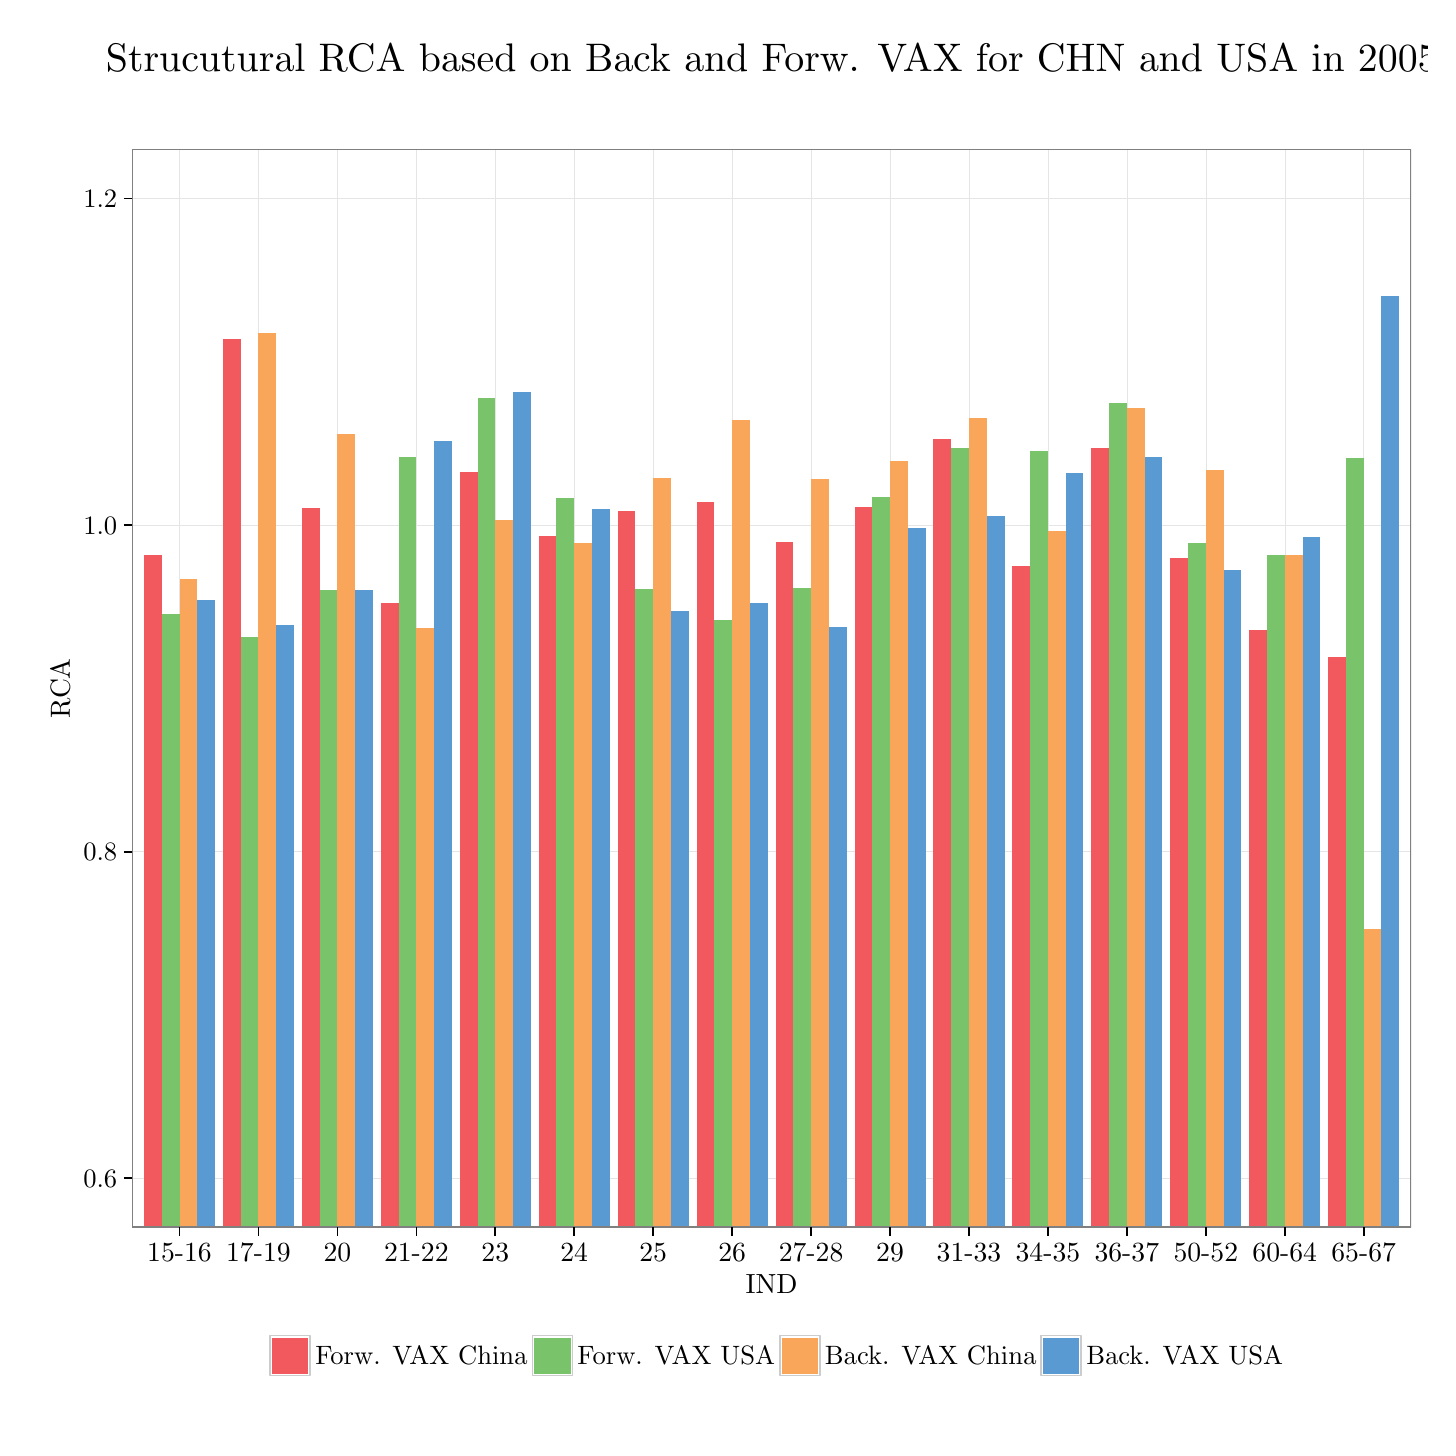
\begin{tikzpicture}[x=1pt,y=1pt]
\definecolor{fillColor}{RGB}{255,255,255}
\path[use as bounding box,fill=fillColor,fill opacity=0.00] (0,0) rectangle (505.89,505.89);
\begin{scope}
\path[clip] (  0.00,  0.00) rectangle (505.89,505.89);
\definecolor{drawColor}{RGB}{255,255,255}
\definecolor{fillColor}{RGB}{255,255,255}

\path[draw=drawColor,line width= 0.6pt,line join=round,line cap=round,fill=fillColor] (  0.00, -0.00) rectangle (505.89,505.89);
\end{scope}
\begin{scope}
\path[clip] ( 37.75, 72.44) rectangle (499.89,461.83);
\definecolor{fillColor}{RGB}{255,255,255}

\path[fill=fillColor] ( 37.75, 72.44) rectangle (499.89,461.83);
\definecolor{drawColor}{gray}{0.90}

\path[draw=drawColor,line width= 0.2pt,line join=round] ( 37.75, 90.14) --
	(499.89, 90.14);

\path[draw=drawColor,line width= 0.2pt,line join=round] ( 37.75,208.13) --
	(499.89,208.13);

\path[draw=drawColor,line width= 0.2pt,line join=round] ( 37.75,326.13) --
	(499.89,326.13);

\path[draw=drawColor,line width= 0.2pt,line join=round] ( 37.75,444.13) --
	(499.89,444.13);

\path[draw=drawColor,line width= 0.2pt,line join=round] ( 54.87, 72.44) --
	( 54.87,461.83);

\path[draw=drawColor,line width= 0.2pt,line join=round] ( 83.39, 72.44) --
	( 83.39,461.83);

\path[draw=drawColor,line width= 0.2pt,line join=round] (111.92, 72.44) --
	(111.92,461.83);

\path[draw=drawColor,line width= 0.2pt,line join=round] (140.45, 72.44) --
	(140.45,461.83);

\path[draw=drawColor,line width= 0.2pt,line join=round] (168.98, 72.44) --
	(168.98,461.83);

\path[draw=drawColor,line width= 0.2pt,line join=round] (197.50, 72.44) --
	(197.50,461.83);

\path[draw=drawColor,line width= 0.2pt,line join=round] (226.03, 72.44) --
	(226.03,461.83);

\path[draw=drawColor,line width= 0.2pt,line join=round] (254.56, 72.44) --
	(254.56,461.83);

\path[draw=drawColor,line width= 0.2pt,line join=round] (283.08, 72.44) --
	(283.08,461.83);

\path[draw=drawColor,line width= 0.2pt,line join=round] (311.61, 72.44) --
	(311.61,461.83);

\path[draw=drawColor,line width= 0.2pt,line join=round] (340.14, 72.44) --
	(340.14,461.83);

\path[draw=drawColor,line width= 0.2pt,line join=round] (368.67, 72.44) --
	(368.67,461.83);

\path[draw=drawColor,line width= 0.2pt,line join=round] (397.19, 72.44) --
	(397.19,461.83);

\path[draw=drawColor,line width= 0.2pt,line join=round] (425.72, 72.44) --
	(425.72,461.83);

\path[draw=drawColor,line width= 0.2pt,line join=round] (454.25, 72.44) --
	(454.25,461.83);

\path[draw=drawColor,line width= 0.2pt,line join=round] (482.77, 72.44) --
	(482.77,461.83);
\definecolor{fillColor}{RGB}{241,89,95}

\path[fill=fillColor] ( 42.03,-263.86) rectangle ( 48.45,315.32);
\definecolor{fillColor}{RGB}{121,195,106}

\path[fill=fillColor] ( 48.45,-263.86) rectangle ( 54.87,294.15);
\definecolor{fillColor}{RGB}{249,166,90}

\path[fill=fillColor] ( 54.87,-263.86) rectangle ( 61.29,306.83);
\definecolor{fillColor}{RGB}{89,154,211}

\path[fill=fillColor] ( 61.29,-263.86) rectangle ( 67.70,298.96);
\definecolor{fillColor}{RGB}{241,89,95}

\path[fill=fillColor] ( 70.56,-263.86) rectangle ( 76.98,393.35);
\definecolor{fillColor}{RGB}{121,195,106}

\path[fill=fillColor] ( 76.98,-263.86) rectangle ( 83.39,285.83);
\definecolor{fillColor}{RGB}{249,166,90}

\path[fill=fillColor] ( 83.39,-263.86) rectangle ( 89.81,395.58);
\definecolor{fillColor}{RGB}{89,154,211}

\path[fill=fillColor] ( 89.81,-263.86) rectangle ( 96.23,289.89);
\definecolor{fillColor}{RGB}{241,89,95}

\path[fill=fillColor] ( 99.08,-263.86) rectangle (105.50,332.46);
\definecolor{fillColor}{RGB}{121,195,106}

\path[fill=fillColor] (105.50,-263.86) rectangle (111.92,302.56);
\definecolor{fillColor}{RGB}{249,166,90}

\path[fill=fillColor] (111.92,-263.86) rectangle (118.34,358.99);
\definecolor{fillColor}{RGB}{89,154,211}

\path[fill=fillColor] (118.34,-263.86) rectangle (124.76,302.51);
\definecolor{fillColor}{RGB}{241,89,95}

\path[fill=fillColor] (127.61,-263.86) rectangle (134.03,298.17);
\definecolor{fillColor}{RGB}{121,195,106}

\path[fill=fillColor] (134.03,-263.86) rectangle (140.45,350.69);
\definecolor{fillColor}{RGB}{249,166,90}

\path[fill=fillColor] (140.45,-263.86) rectangle (146.87,288.99);
\definecolor{fillColor}{RGB}{89,154,211}

\path[fill=fillColor] (146.87,-263.86) rectangle (153.29,356.46);
\definecolor{fillColor}{RGB}{241,89,95}

\path[fill=fillColor] (156.14,-263.86) rectangle (162.56,345.33);
\definecolor{fillColor}{RGB}{121,195,106}

\path[fill=fillColor] (162.56,-263.86) rectangle (168.98,372.23);
\definecolor{fillColor}{RGB}{249,166,90}

\path[fill=fillColor] (168.98,-263.86) rectangle (175.39,327.86);
\definecolor{fillColor}{RGB}{89,154,211}

\path[fill=fillColor] (175.39,-263.86) rectangle (181.81,374.15);
\definecolor{fillColor}{RGB}{241,89,95}

\path[fill=fillColor] (184.67,-263.86) rectangle (191.08,322.36);
\definecolor{fillColor}{RGB}{121,195,106}

\path[fill=fillColor] (191.08,-263.86) rectangle (197.50,336.08);
\definecolor{fillColor}{RGB}{249,166,90}

\path[fill=fillColor] (197.50,-263.86) rectangle (203.92,319.78);
\definecolor{fillColor}{RGB}{89,154,211}

\path[fill=fillColor] (203.92,-263.86) rectangle (210.34,331.97);
\definecolor{fillColor}{RGB}{241,89,95}

\path[fill=fillColor] (213.19,-263.86) rectangle (219.61,331.14);
\definecolor{fillColor}{RGB}{121,195,106}

\path[fill=fillColor] (219.61,-263.86) rectangle (226.03,303.11);
\definecolor{fillColor}{RGB}{249,166,90}

\path[fill=fillColor] (226.03,-263.86) rectangle (232.45,343.16);
\definecolor{fillColor}{RGB}{89,154,211}

\path[fill=fillColor] (232.45,-263.86) rectangle (238.87,295.14);
\definecolor{fillColor}{RGB}{241,89,95}

\path[fill=fillColor] (241.72,-263.86) rectangle (248.14,334.52);
\definecolor{fillColor}{RGB}{121,195,106}

\path[fill=fillColor] (248.14,-263.86) rectangle (254.56,291.98);
\definecolor{fillColor}{RGB}{249,166,90}

\path[fill=fillColor] (254.56,-263.86) rectangle (260.98,364.12);
\definecolor{fillColor}{RGB}{89,154,211}

\path[fill=fillColor] (260.98,-263.86) rectangle (267.39,298.09);
\definecolor{fillColor}{RGB}{241,89,95}

\path[fill=fillColor] (270.25,-263.86) rectangle (276.67,320.14);
\definecolor{fillColor}{RGB}{121,195,106}

\path[fill=fillColor] (276.67,-263.86) rectangle (283.08,303.41);
\definecolor{fillColor}{RGB}{249,166,90}

\path[fill=fillColor] (283.08,-263.86) rectangle (289.50,342.68);
\definecolor{fillColor}{RGB}{89,154,211}

\path[fill=fillColor] (289.50,-263.86) rectangle (295.92,289.48);
\definecolor{fillColor}{RGB}{241,89,95}

\path[fill=fillColor] (298.77,-263.86) rectangle (305.19,332.80);
\definecolor{fillColor}{RGB}{121,195,106}

\path[fill=fillColor] (305.19,-263.86) rectangle (311.61,336.16);
\definecolor{fillColor}{RGB}{249,166,90}

\path[fill=fillColor] (311.61,-263.86) rectangle (318.03,349.44);
\definecolor{fillColor}{RGB}{89,154,211}

\path[fill=fillColor] (318.03,-263.86) rectangle (324.45,325.01);
\definecolor{fillColor}{RGB}{241,89,95}

\path[fill=fillColor] (327.30,-263.86) rectangle (333.72,357.43);
\definecolor{fillColor}{RGB}{121,195,106}

\path[fill=fillColor] (333.72,-263.86) rectangle (340.14,354.16);
\definecolor{fillColor}{RGB}{249,166,90}

\path[fill=fillColor] (340.14,-263.86) rectangle (346.56,364.97);
\definecolor{fillColor}{RGB}{89,154,211}

\path[fill=fillColor] (346.56,-263.86) rectangle (352.98,329.34);
\definecolor{fillColor}{RGB}{241,89,95}

\path[fill=fillColor] (355.83,-263.86) rectangle (362.25,311.51);
\definecolor{fillColor}{RGB}{121,195,106}

\path[fill=fillColor] (362.25,-263.86) rectangle (368.67,352.82);
\definecolor{fillColor}{RGB}{249,166,90}

\path[fill=fillColor] (368.67,-263.86) rectangle (375.08,323.98);
\definecolor{fillColor}{RGB}{89,154,211}

\path[fill=fillColor] (375.08,-263.86) rectangle (381.50,344.97);
\definecolor{fillColor}{RGB}{241,89,95}

\path[fill=fillColor] (384.36,-263.86) rectangle (390.77,354.11);
\definecolor{fillColor}{RGB}{121,195,106}

\path[fill=fillColor] (390.77,-263.86) rectangle (397.19,370.34);
\definecolor{fillColor}{RGB}{249,166,90}

\path[fill=fillColor] (397.19,-263.86) rectangle (403.61,368.32);
\definecolor{fillColor}{RGB}{89,154,211}

\path[fill=fillColor] (403.61,-263.86) rectangle (410.03,350.87);
\definecolor{fillColor}{RGB}{241,89,95}

\path[fill=fillColor] (412.88,-263.86) rectangle (419.30,314.08);
\definecolor{fillColor}{RGB}{121,195,106}

\path[fill=fillColor] (419.30,-263.86) rectangle (425.72,319.63);
\definecolor{fillColor}{RGB}{249,166,90}

\path[fill=fillColor] (425.72,-263.86) rectangle (432.14,346.23);
\definecolor{fillColor}{RGB}{89,154,211}

\path[fill=fillColor] (432.14,-263.86) rectangle (438.56,309.74);
\definecolor{fillColor}{RGB}{241,89,95}

\path[fill=fillColor] (441.41,-263.86) rectangle (447.83,288.29);
\definecolor{fillColor}{RGB}{121,195,106}

\path[fill=fillColor] (447.83,-263.86) rectangle (454.25,315.23);
\definecolor{fillColor}{RGB}{249,166,90}

\path[fill=fillColor] (454.25,-263.86) rectangle (460.67,315.22);
\definecolor{fillColor}{RGB}{89,154,211}

\path[fill=fillColor] (460.67,-263.86) rectangle (467.08,321.74);
\definecolor{fillColor}{RGB}{241,89,95}

\path[fill=fillColor] (469.94,-263.86) rectangle (476.36,278.44);
\definecolor{fillColor}{RGB}{121,195,106}

\path[fill=fillColor] (476.36,-263.86) rectangle (482.77,350.36);
\definecolor{fillColor}{RGB}{249,166,90}

\path[fill=fillColor] (482.77,-263.86) rectangle (489.19,180.06);
\definecolor{fillColor}{RGB}{89,154,211}

\path[fill=fillColor] (489.19,-263.86) rectangle (495.61,408.89);
\definecolor{drawColor}{gray}{0.50}

\path[draw=drawColor,line width= 0.6pt,line join=round,line cap=round] ( 37.75, 72.44) rectangle (499.89,461.83);
\end{scope}
\begin{scope}
\path[clip] (  0.00,  0.00) rectangle (505.89,505.89);
\definecolor{drawColor}{RGB}{0,0,0}

\node[text=drawColor,anchor=base east,inner sep=0pt, outer sep=0pt, scale=  0.96] at ( 32.35, 86.83) {0.6};

\node[text=drawColor,anchor=base east,inner sep=0pt, outer sep=0pt, scale=  0.96] at ( 32.35,204.83) {0.8};

\node[text=drawColor,anchor=base east,inner sep=0pt, outer sep=0pt, scale=  0.96] at ( 32.35,322.83) {1.0};

\node[text=drawColor,anchor=base east,inner sep=0pt, outer sep=0pt, scale=  0.96] at ( 32.35,440.83) {1.2};
\end{scope}
\begin{scope}
\path[clip] (  0.00,  0.00) rectangle (505.89,505.89);
\definecolor{drawColor}{RGB}{0,0,0}

\path[draw=drawColor,line width= 0.6pt,line join=round] ( 34.75, 90.14) --
	( 37.75, 90.14);

\path[draw=drawColor,line width= 0.6pt,line join=round] ( 34.75,208.13) --
	( 37.75,208.13);

\path[draw=drawColor,line width= 0.6pt,line join=round] ( 34.75,326.13) --
	( 37.75,326.13);

\path[draw=drawColor,line width= 0.6pt,line join=round] ( 34.75,444.13) --
	( 37.75,444.13);
\end{scope}
\begin{scope}
\path[clip] (  0.00,  0.00) rectangle (505.89,505.89);
\definecolor{drawColor}{RGB}{0,0,0}

\path[draw=drawColor,line width= 0.6pt,line join=round] ( 54.87, 69.44) --
	( 54.87, 72.44);

\path[draw=drawColor,line width= 0.6pt,line join=round] ( 83.39, 69.44) --
	( 83.39, 72.44);

\path[draw=drawColor,line width= 0.6pt,line join=round] (111.92, 69.44) --
	(111.92, 72.44);

\path[draw=drawColor,line width= 0.6pt,line join=round] (140.45, 69.44) --
	(140.45, 72.44);

\path[draw=drawColor,line width= 0.6pt,line join=round] (168.98, 69.44) --
	(168.98, 72.44);

\path[draw=drawColor,line width= 0.6pt,line join=round] (197.50, 69.44) --
	(197.50, 72.44);

\path[draw=drawColor,line width= 0.6pt,line join=round] (226.03, 69.44) --
	(226.03, 72.44);

\path[draw=drawColor,line width= 0.6pt,line join=round] (254.56, 69.44) --
	(254.56, 72.44);

\path[draw=drawColor,line width= 0.6pt,line join=round] (283.08, 69.44) --
	(283.08, 72.44);

\path[draw=drawColor,line width= 0.6pt,line join=round] (311.61, 69.44) --
	(311.61, 72.44);

\path[draw=drawColor,line width= 0.6pt,line join=round] (340.14, 69.44) --
	(340.14, 72.44);

\path[draw=drawColor,line width= 0.6pt,line join=round] (368.67, 69.44) --
	(368.67, 72.44);

\path[draw=drawColor,line width= 0.6pt,line join=round] (397.19, 69.44) --
	(397.19, 72.44);

\path[draw=drawColor,line width= 0.6pt,line join=round] (425.72, 69.44) --
	(425.72, 72.44);

\path[draw=drawColor,line width= 0.6pt,line join=round] (454.25, 69.44) --
	(454.25, 72.44);

\path[draw=drawColor,line width= 0.6pt,line join=round] (482.77, 69.44) --
	(482.77, 72.44);
\end{scope}
\begin{scope}
\path[clip] (  0.00,  0.00) rectangle (505.89,505.89);
\definecolor{drawColor}{RGB}{0,0,0}

\node[text=drawColor,anchor=base,inner sep=0pt, outer sep=0pt, scale=  1.00] at ( 54.87, 60.15) {15-16};

\node[text=drawColor,anchor=base,inner sep=0pt, outer sep=0pt, scale=  1.00] at ( 83.39, 60.15) {17-19};

\node[text=drawColor,anchor=base,inner sep=0pt, outer sep=0pt, scale=  1.00] at (111.92, 60.15) {20};

\node[text=drawColor,anchor=base,inner sep=0pt, outer sep=0pt, scale=  1.00] at (140.45, 60.15) {21-22};

\node[text=drawColor,anchor=base,inner sep=0pt, outer sep=0pt, scale=  1.00] at (168.98, 60.15) {23};

\node[text=drawColor,anchor=base,inner sep=0pt, outer sep=0pt, scale=  1.00] at (197.50, 60.15) {24};

\node[text=drawColor,anchor=base,inner sep=0pt, outer sep=0pt, scale=  1.00] at (226.03, 60.15) {25};

\node[text=drawColor,anchor=base,inner sep=0pt, outer sep=0pt, scale=  1.00] at (254.56, 60.15) {26};

\node[text=drawColor,anchor=base,inner sep=0pt, outer sep=0pt, scale=  1.00] at (283.08, 60.15) {27-28};

\node[text=drawColor,anchor=base,inner sep=0pt, outer sep=0pt, scale=  1.00] at (311.61, 60.15) {29};

\node[text=drawColor,anchor=base,inner sep=0pt, outer sep=0pt, scale=  1.00] at (340.14, 60.15) {31-33};

\node[text=drawColor,anchor=base,inner sep=0pt, outer sep=0pt, scale=  1.00] at (368.67, 60.15) {34-35};

\node[text=drawColor,anchor=base,inner sep=0pt, outer sep=0pt, scale=  1.00] at (397.19, 60.15) {36-37};

\node[text=drawColor,anchor=base,inner sep=0pt, outer sep=0pt, scale=  1.00] at (425.72, 60.15) {50-52};

\node[text=drawColor,anchor=base,inner sep=0pt, outer sep=0pt, scale=  1.00] at (454.25, 60.15) {60-64};

\node[text=drawColor,anchor=base,inner sep=0pt, outer sep=0pt, scale=  1.00] at (482.77, 60.15) {65-67};
\end{scope}
\begin{scope}
\path[clip] (  0.00,  0.00) rectangle (505.89,505.89);
\definecolor{drawColor}{RGB}{0,0,0}

\node[text=drawColor,anchor=base,inner sep=0pt, outer sep=0pt, scale=  1.00] at (268.82, 48.46) {IND};
\end{scope}
\begin{scope}
\path[clip] (  0.00,  0.00) rectangle (505.89,505.89);
\definecolor{drawColor}{RGB}{0,0,0}

\node[text=drawColor,rotate= 90.00,anchor=base,inner sep=0pt, outer sep=0pt, scale=  1.00] at ( 15.29,267.13) {RCA};
\end{scope}
\begin{scope}
\path[clip] (  0.00,  0.00) rectangle (505.89,505.89);
\definecolor{fillColor}{RGB}{255,255,255}

\path[fill=fillColor] ( 79.79, 14.54) rectangle (457.85, 37.53);
\end{scope}
\begin{scope}
\path[clip] (  0.00,  0.00) rectangle (505.89,505.89);
\definecolor{drawColor}{gray}{0.80}
\definecolor{fillColor}{RGB}{255,255,255}

\path[draw=drawColor,line width= 0.6pt,line join=round,line cap=round,fill=fillColor] ( 87.67, 18.80) rectangle (102.12, 33.26);
\end{scope}
\begin{scope}
\path[clip] (  0.00,  0.00) rectangle (505.89,505.89);
\definecolor{fillColor}{RGB}{241,89,95}

\path[fill=fillColor] ( 88.38, 19.52) rectangle (101.41, 32.55);
\end{scope}
\begin{scope}
\path[clip] (  0.00,  0.00) rectangle (505.89,505.89);
\definecolor{drawColor}{gray}{0.80}
\definecolor{fillColor}{RGB}{255,255,255}

\path[draw=drawColor,line width= 0.6pt,line join=round,line cap=round,fill=fillColor] (182.41, 18.80) rectangle (196.87, 33.26);
\end{scope}
\begin{scope}
\path[clip] (  0.00,  0.00) rectangle (505.89,505.89);
\definecolor{fillColor}{RGB}{121,195,106}

\path[fill=fillColor] (183.12, 19.52) rectangle (196.16, 32.55);
\end{scope}
\begin{scope}
\path[clip] (  0.00,  0.00) rectangle (505.89,505.89);
\definecolor{drawColor}{gray}{0.80}
\definecolor{fillColor}{RGB}{255,255,255}

\path[draw=drawColor,line width= 0.6pt,line join=round,line cap=round,fill=fillColor] (271.82, 18.80) rectangle (286.28, 33.26);
\end{scope}
\begin{scope}
\path[clip] (  0.00,  0.00) rectangle (505.89,505.89);
\definecolor{fillColor}{RGB}{249,166,90}

\path[fill=fillColor] (272.54, 19.52) rectangle (285.57, 32.55);
\end{scope}
\begin{scope}
\path[clip] (  0.00,  0.00) rectangle (505.89,505.89);
\definecolor{drawColor}{gray}{0.80}
\definecolor{fillColor}{RGB}{255,255,255}

\path[draw=drawColor,line width= 0.6pt,line join=round,line cap=round,fill=fillColor] (366.27, 18.80) rectangle (380.73, 33.26);
\end{scope}
\begin{scope}
\path[clip] (  0.00,  0.00) rectangle (505.89,505.89);
\definecolor{fillColor}{RGB}{89,154,211}

\path[fill=fillColor] (366.98, 19.52) rectangle (380.02, 32.55);
\end{scope}
\begin{scope}
\path[clip] (  0.00,  0.00) rectangle (505.89,505.89);
\definecolor{drawColor}{RGB}{0,0,0}

\node[text=drawColor,anchor=base west,inner sep=0pt, outer sep=0pt, scale=  0.96] at (103.93, 22.72) {Forw. VAX China};
\end{scope}
\begin{scope}
\path[clip] (  0.00,  0.00) rectangle (505.89,505.89);
\definecolor{drawColor}{RGB}{0,0,0}

\node[text=drawColor,anchor=base west,inner sep=0pt, outer sep=0pt, scale=  0.96] at (198.67, 22.72) {Forw. VAX USA};
\end{scope}
\begin{scope}
\path[clip] (  0.00,  0.00) rectangle (505.89,505.89);
\definecolor{drawColor}{RGB}{0,0,0}

\node[text=drawColor,anchor=base west,inner sep=0pt, outer sep=0pt, scale=  0.96] at (288.08, 22.72) {Back. VAX China};
\end{scope}
\begin{scope}
\path[clip] (  0.00,  0.00) rectangle (505.89,505.89);
\definecolor{drawColor}{RGB}{0,0,0}

\node[text=drawColor,anchor=base west,inner sep=0pt, outer sep=0pt, scale=  0.96] at (382.53, 22.72) {Back. VAX USA};
\end{scope}
\begin{scope}
\path[clip] (  0.00,  0.00) rectangle (505.89,505.89);
\definecolor{drawColor}{RGB}{0,0,0}

\node[text=drawColor,anchor=base west,inner sep=0pt, outer sep=0pt, scale=  1.44] at ( 28.26,489.97) {Strucutural RCA based on  Back and Forw. VAX for CHN and USA in 2005};
\end{scope}
\end{tikzpicture}
